\chapter{Introduction}
\label{Chap:intro}

% epigraph (done: 2021年8月13日17:13:54)
\setlength{\unitlength}{1pt}
\setlength{\epigraphwidth}{11cm}
\epigraph{Historians may re-examine the mistakes of the past in the hope of providing warning for the future, but at the same time caution their readers to preserve what is of value. \cite{HuangRay19811ayo}}{--- Ray Huang\\ \textit{1587, a Year of No Significance (1981)}}

% introduction and purpose (done 2021年7月9日14:34:47)
The world is made up of various substances, and even the same substance can be in different \textit{phases}. Besides finding new particles and materials, discovering new phases of matter is also an essential subject of physics. When discovered phases of matter accumulating, how to classify, explain and understand them from the perspective of microscopic theory gradually becomes the core topic of physics. This thesis will introduce a new quantum phase of ultracold atoms, i.e. the quantum liquid droplet. Correspondingly, the microscopic theory about the beyond mean-field effect, Lee-Huang-Yang (LHY) correction\cite{lee1957}, will be discussed detailedly in the latter chapters. This chapter will introduce the history of the topic developed in recent years and its influence on other fields. I try to offer readers a broader picture for a better understanding of quantum liquid droplet.

% arrangement of this chapter (done 2021年7月9日14:34:24)
This chapter is arranged as follows: section \ref{sec:intro-background} introduces our research goal, the quantum droplet. By introducing some background knowledge and researches from related fields, I try to discuss why we study the Na-Rb BEC-mixture droplet. In section \ref{sec:intro-overview}, I will review my research journey in these two years, trying to retrieve a storyline of our struggling instead of only the perfect developed ending. Section \ref{sec:intro-LHY} will discuss the core concepts of LHY correction and its history, as a precursor of Chapter \ref{Chap:theory}. Finally, section \ref{sec:intro-outline} offers the arrangement of the whole thesis.

%%%%%%%%%%%%%  sec:intro-background  %%%%%%%%%%%%%%%%
\section{Why quantum liquid droplets?}
\label{sec:intro-background}

% start from classical droplet
Before answering the question on the title, i.e. about the \textit{quantum} liquid droplet, we first draw some attention to the \textit{classical} liquid-gas phase transition. As shown in Fig. \ref{Classical_and_quantum_droplet}, a classical gas can be regarded as a bunch of interacting particles. Typically, we use the Van der Waals interaction as a good approximation, i.e. a hard-core (repulsion) plus a long-range attractive potential. By adding this inter-particle interaction to the equation of state, we get the famous Van der Waals equation:
\begin{equation}
\label{VdW equation}
(P+a\frac{n^2}{V^2})(V-bn)=nRT
\end{equation}
where the ``\(b\)'' factor represents the size of the hardcore, since the effective volume of sample is enlarged, and ``\(a\)'' shows the attractive interaction between particles which reduces the pressure of the sample. This equation implies the liquid-gas phase transition when the temperature is lowering down to a specific \(T_C=\frac{8a}{27Rb}\). The detailed analysis could be found in the textbook \cite{Cowan2005}. So, here we only focus on the physics picture. For a liquid phase sample, as shown in Fig. \ref{Classical_and_quantum_droplet} right-top panel, the particles are squeezed to their hard-cores touching to each other. This features the incompressibility of a liquid sample. The kinetic energy of particles maintain their mobility, and due to easily exchange of particle position, we still have a fluid instead of a solid phase. In another perspective, the attractive range of particles overlapping with each other indicates a strong correlation. One particle could affect many other particles. We call this a long-range interaction system, which is typically hard to tackle. So, even with full knowledge of its microscopic equation, sometimes the behaviour of liquid can still amaze us, such as Non-Newtonian fluid or liquid crystal.

% add classical and quantum droplet comparison figure (done: 2021年7月29日19:30:32)
\begin{figure}[htbp]
\begin{center}
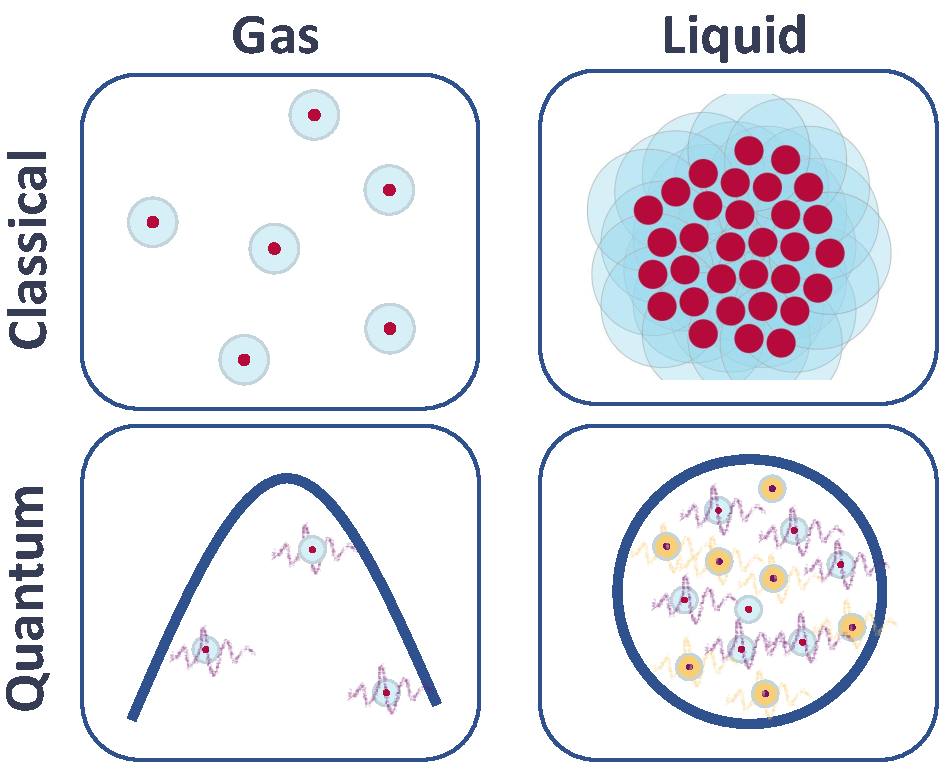
\includegraphics [width = 0.8 \linewidth]{Classical_and_quantum_droplet.pdf}
\end{center}
\caption[Comparison between classical and quantum liquid droplet]{Classical and quantum Liquid-gas phase transition. The upper panel shows a classical liquid-gas phase transition, which is explained by the famous Van der Waals equation. With this theory, particles interact with short-range hardcore (red solid part) and long-range attraction (light-blue outer). When the temperature lowers to the critical temperature, the sample undergoes a phase transition to be a liquid. As shown in the upper-right block, particles stay close to each other with inter-particle distance around the size of its hardcore. Meanwhile, their long-range parts overlap, showing a strongly correlated feature. For the lower panel, we draw the quantum liquid-gas phase transition for a BEC mixture sample. The thick blue line represents the shared wave function for the condensate part. The particle with a de-Broglie wave-packet represents the quantum depletion due to interaction excitation from the condensate. The right-bottom one shows the BEC mixture liquid droplet, which is the main topic of this thesis.}
\label{Classical_and_quantum_droplet}
\end{figure}

%%%%%%%%%%%%%%%%%%%%%%%%%%%%%%%%%%%%%%%%%%%%%%%%%%%%%%%%
% to quantum matter, quantum gas sample (done: 2021年8月16日21:54:08)
Then, a question arises naturally for cold atom physicists: what about a quantum system? Is there any liquid phase for a Bose-Einstein condensate? A positive answer is made by Petrov in 2015 \cite{petrov2015}. For a dilute ultracold BEC mixture, we do have a liquid phase. However, this kind of liquid is dramatically different from the classical one. First, it is a zero-temperature sample, which means the thermal fluctuation is suppressed. Second, the sample is still dilute with an interparticle distance larger than 100 nm (interacting range typical around several nm). This indicates the system should be still in a weak-interacting case. Finally, quantum fluctuation shows its essential role. However, instead of serving as a driven force for mobility, the quantum fluctuation cures the sample's collapse or implosion. To study this sample, we could understand more profound the beyond mean-field correction of this many-body system.

% introduce quantum depletion and call droplet (done 2021年7月26日17:53:24)
As a new field in ultracold atoms, quantum liquid droplets originated from the deep understanding of the beyond mean-field theory of Bose-Einstein condensate (BEC) and from an innovative and careful extrapolation of textbook theory. In the past 25 years discovery of ultracold gases, mean-field theory (MF theory), as the zero-order solution of a many-body system, dominates the explanation of most phenomena. Especially for Bose-Einstein condensate, it explains plenty of interesting experiment observations, including the state of the equation for in-trap sample, excitation mode, dark soliton, bright solution, BEC collapse and so on. This zero-order approximation considers the condensates as a single wave-function \(\Psi\), which is based on the observation that most atoms share the same ground state, i.e. the \(k=0\) state (for uniform case). However, particles from the condensate could be excited to a finite momentum state due to the interaction between particles. From the microscopic theory of condensate, these particles with \(k>0\) have a fraction of order of \(\sqrt{na^3}\) compared to the condensate part, which occupies a tiny portion when the interaction is weak. Thus, we call it quantum depletion. This tiny portion brings only a tiny correction to its ground-state energy; so, people typical ignore its effect in most cases. However, things get incredibly different in the quantum liquid droplet; here, quantum depletion plays a vital role because the depletion part contributes a competitive energy scale to the mean-field energy. 

% what is quantum droplet? (done 2021年7月26日21:44:05)
Proposed by Petrov in 2015 \cite{petrov2015}, a BEC mixture with overall negative mean-field energy could survive from collapsing and form a quantum droplet. Surprisingly, this theory was first used to explain the self-bound behaviour in the dipolar gas \cite{ferrier2016Liquid,chomaz2016}. Then in 2018, Leticia group \cite{cabrera2018quantum} discovered the first double BEC droplet in a spin mixture of \(^{39}\)K. These two distinctive systems are related to the same theoretical explanation, showing the ubiquity that how important role for the LHY correction in ultracold atoms. For both cases, the mean-field energy approaches zero and is tuned by a Feshbach resonance for an inter-species \(s\)-wave contact interaction. Meanwhile, the LHY correction remains a positive value and grows even fast than the mean-field one when the density of the sample increasing. So, it cures the mean-field collapse. The difference between a dipolar droplet and a mixture BEC droplet is the inter-particle interaction type: for dipolar case, the interaction is anisotropic, which renders an anisotropic sample as well; however, for the BEC mixture case, thanks to the isotropic interaction, the sample shows a perfect spherical shape.

% droplet in different system (done: 2021年8月15日11:40:20)
As mentioned before, Petrov's theory was first used to the dipolar droplet \cite{ferrier2016Liquid,chomaz2016}, which is made of magnetic atoms with anisotropic interaction. Then in 2018, two groups \cite{cabrera2018quantum,semeghini2018self} produced the double BEC droplet exactly matching Petrov's original proposal. Latter, many works sprung up, in both experiment and theory. Leticia's group produce the droplet in a wave-guide \cite{cheiney2018bright}, in which they study the bright soliton to the droplet phase transition. From the low-dimension point of view, many theoretical proposals are developing, including \cite{petrov2016ultradilute,Ilg2018,Cui2021}. In another point of view, i.e. the gas phase sample with near-zero mean-field energy, theory \cite{Jorgensen2018}, and experiment \cite{skov2020} study the changing of monopole mode of an LHY gas. 

% why we study droplet? (done: 2021年8月15日19:44:00)
The initial purpose of our research was to make a heteronuclear droplet. With a rough calculation, we estimate its lifetime could reach about 100 ms, enabling us to do further research such as its excitation spectrum and the self evaporation. However, later we find the lifetime of the sample limited to 10 ms level. We attribute this to the large three-body loss between two species. Then, we have to turn our research goal to study the LHY effects in a double BEC of $^{23}$Na and $^{87}$Rb atoms in two different ways. First, we build the heteronuclear quantum liquid droplet in free space with more than $10^4$ atoms when the interspecies Na-Rb scattering length is tuned into the mean-field collapse regime. Under optimized conditions, a low-number-density droplet with a lifetime exceeding the observation time is observed. We also investigate the liquid-to-gas phase transition and obtain the critical atom numbers at the phase boundary. Second, we measure the release energies of two types of gas-phase mixtures, the pure in-trap gas and the gas formed after a droplet crosses the liquid-to-gas transition, and observe their opposite dependence on the interaction strength.  With calculations based on extended Gross-Pitaevskii equations (eGPEs), our results confirm the crucial contribution of $E_{\rm LHY}$ and its effects in stabilizing the heteronuclear double BEC far into the mean-field collapse region.

\section{Thesis Overview}
\label{sec:intro-overview}
% a introduction of this section (done: 2021年8月15日19:59:19)
In this section, instead of demonstrating our research result of the heteronuclear droplet, I try to tell the story of how we were stuck in each step and how we solved problems. I summarize what we learnt from the research process, such as ``be wary of every unverified number''. I hope this complementary material can serve as a lesson for myself and the readers.

% About ToF in low magnetic field (done: 2021年8月15日20:35:52)
Our experiment of the droplet started in February of 2018. We first test the miscibility and immiscibility of a mixture BEC sample near the 347 G Feshbach resonance. Ref. \cite{wang2015double} tested this feature after time-of-flight (ToF) in a low magnetic field, which introduces deviation on the measurement of phase separation boundary. The ToF in a low magnetic field changes the scattering length between Na and Rb from the target value (such as -50 \(a_0\)) to the background one (i.e. 76 \(a_0\)). This renders the mixture BEC immiscible, whatever its original miscibility in the high magnetic field, and causes a shift of the separation boundary. So, we tried to test the miscibility of the BEC mixture with different duration (\(\Delta\) ms) between quenching the magnetic field down and releasing the optical trap (as shown in Fig. \ref{ToF_dBEC_highBfield}). By controlling this duration, we test the dynamics of the BEC mixture in the ToF process with different interspecies interactions. For example, we hold the magnetic field at 354.1 G, where the scattering length between Na and Rb is 26 \(a_0\). The sample is in a miscible phase. However, as shown in Fig. \ref{ToF_dBEC_highBfield}, with \(\Delta<\) 4 ms, an unmistakable immiscible signal shows up.

% ToF for a BEC mixture with different duration in high magnetic field
% (done 2021年8月16日10:11:48)
\begin{figure}[htb]
\begin{center}
\includegraphics [width = 1 \linewidth]{ToF_dBEC_highBfield.pdf}
\end{center}
\caption[ToF of Na-Rb BEC mixture under high magnetic field]{The upper panel shows the time sequence of testing the dynamic of a mixture BEC sample ToF under a high magnetic field. We first shut down the optical dipole trap, and the sample will free fall in the free space. Then, we hold the magnetic field for \(\Delta\) ms, where the interspecies interaction is unchanged. Finally, to do a typical absorption image, we quench the magnetic field to several Gauss. We test different \(\Delta\), however, keep duration between image and the timing we turn off the optical trap. The bottom panel shows the absorption images of Na and Rb. The magnetic field is held at 354.1 G ($a_{\rm Na-Rb}=26 a_0$) for different duration $\Delta$ ms. With a shorter duration, the immiscibility becomes more severe.}
\label{ToF_dBEC_highBfield}
\end{figure}

% use the new method to detect the MF collapse (done: 2021年8月16日22:16:30)
Then we try to approach the mean-field (MF) collapse region in the mixture BEC sample. With the above mentioned ToF method under a high magnetic field, the detection can reflect unaffected miscibility of the mixture sample. We use $\Delta=10$ ms ToF inside the high magnetic field, which lowers down the density of the sample and releases its interaction energy. Then it is safe to switch off the magnetic field and take the image in a low field. The imaging timing for Na(Rb) is 13(18) ms after switching off the optical trap. By scanning the interspecies interaction, as shown in Fig. \ref{dBEC_miscibility}, we test the behaviour of the sample from +12.45 $a_0$ to -63.75 $a_0$. When gradually lower down the scattering length, the sample's size suddenly shrinks at about -44 a0. Loss of atoms number also increases as the Optical depth of the sample get shallower. At that time, we only know about the collapse of the BEC, such as observed in Li~\cite{donley2001}. For the Na-Rb mixture, the MF collapse point is about -60 a0. So, we thought that should be a collapse of the mixture sample. This collapse increases the density of the sample and causes a severe three-body loss.

% double BEC miscibility (done: 2021年8月16日10:37:18)
\begin{figure}[htb]
\begin{center}
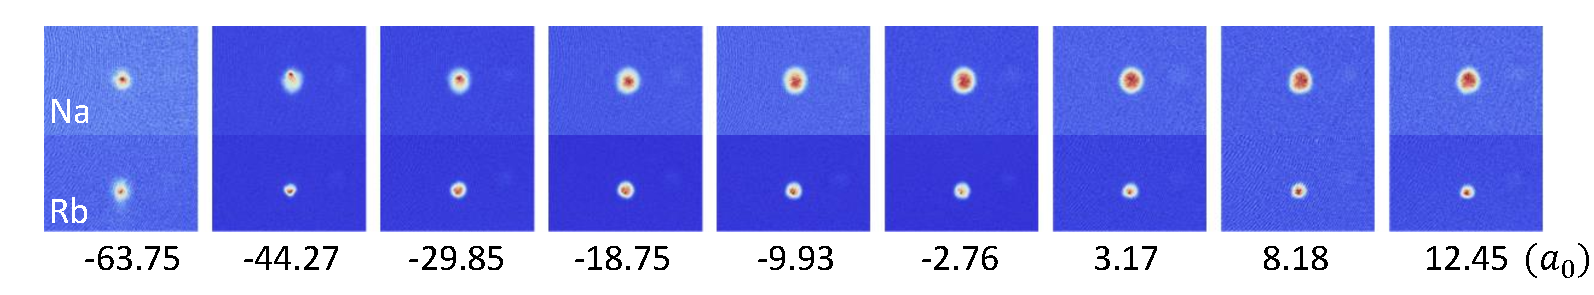
\includegraphics [width = 1 \linewidth]{dBEC_miscibility .pdf}
\end{center}
\caption[Na-Rb BEC mixture with various inter-species interaction]{With method introduced in Fig. \ref{ToF_dBEC_highBfield}, we scan the interspecies interaction to probe the miscibility of mixture BEC sample. The ToF duration in free space for Na(Rb) is 13(18) ms. From right to left, with $a_{\rm Na-Rb}$ gradually decreasing, the size of both Na and Rb shrinks. Moreover, a severe loss is detected for $a_{\rm Na-Rb}=-63.8 a_0$}
\label{dBEC_miscibility}
\end{figure}

% start droplet experiment (done: 2021年8月16日22:17:25)
Then, we notice Petrov's paper \cite{petrov2015}, in which he described a stabilization mechanism that could avoid the MF collapse by the so-called LHY correction. Meanwhile, we found Leticia's paper \cite{cabrera2018quantum} showing the experimental study of the ${}^{39}$K droplet. This work encourages us to re-do the experiment mentioned above again and try to find the droplet signal. So, that is the start point of our experiment. Our goal is to build the first hetero-nuclear droplet made of a mixture Na-Rb BEC.

% droplet in low field image (done: 2021年8月17日11:12:41)
At the very beginning, we only have absorption image in the low magnetic field, which considerably limit our ability to detect the droplet signal. Because quantum droplet's size is relatively small, typically less than 2-3 \(\mu m\). With this limited image method, we have to detect the signal after a long ToF. As we already know, the dynamics during the ToF would severely affect the sample's shape and size. We thus choose to do the ToF under 350 G magnetic field for 5 ms first, then switch down the magnetic field. After 8(13) ms ToF in the low magnetic field, we do a Na(Rb) absorption image. As shown in Fig. \ref{LowField_droplet}, we measure the sample's size and number. When the magnetic field is higher than 352 G, i.e. around \(a_{\rm Na-Rb}=0\), both Na and Rb show a constant size and number. When the magnetic field gradually decrease to 350.4 G, i.e. about -40 \(a_0\), the size of Na decreases; meanwhile, Rb size is almost unchanged. This phenomenon can be understood that Na has absorbed into Rb thanks to the miscible and attractive interaction. When the magnetic field decreases further, a severe loss shows up for both Na and Rb, mainly due to the three-body loss happening when the density gets high. Then when the magnetic field is across 350 G, sizes of both Na and Rb increase sharply upon the magnetic field. Here, we already find this abnormal expansion velocity of the sample. However, the explanation could be either three-body loss(heating) in a droplet sample or just BEC collapsing, which is hard to distinguish them.

% Low field image for droplet signal (done 2021年8月17日11:13:55)
\begin{figure}[htbp]
\begin{center}
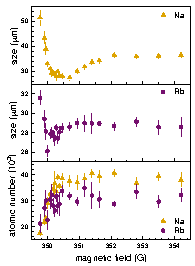
\includegraphics [width = 0.6 \linewidth]{LowField_droplet.pdf}
\end{center}
\caption[Try to detect droplet signal by low field image]{This figure shows our try at detecting droplet signals with a low-magnetic field absorption image. With the magnetic field decrease from 352 G to 350 G, we can see an apparent decrease in the size of both Na and Rb. This is thanks to the inter-species attractive interaction. Then, with a further decrease of the magnetic field, we see steep inflation of sample size and severe loss.}
\label{LowField_droplet}
\end{figure}

% problem with low field image (done 2021年8月17日11:34:04)
With this measurement, we cannot make conclusion that we catch the signal of droplet. Whatever, we spent only two weeks doing the fast test and making the decision, which is judicious from the current point of view. Besides the above mentioned reasons, we have to suspect the destructive dynamics of the sample during the ToF when the magnetic field switching down. Because the droplet sample have a density even 10 times larger than a typical BEC sample, we have to treat this ToF process very carefully. So, what we need is a new image method which can directly capture the sample under a high magnetic field (around 350 G). We stop our experiment and try to design a image method working under high magnetic field. First, we want to try the Faraday image. We do the calculation, trying to find the rotation angle for our sample. However the calculation shows that we need an EMCCD to get enough SNR, which is out of our afford. So we turn back to try the absorption image under a high magnetic field. There were two problems: we need to find a cycling (or almost-cycling) transition under 350 G; another is we need to handle the sample with extremely high optical density (OD), around 10 to 50 for the Rb sample. We calculate and conceive all possible image scheme, such as two examples shown in Fig. \ref{image_scheme_II}. We first try a $90\%$ almost-cycling transition (shown in (a) of Fig. \ref{image_scheme_II}), then we turn to the other one since even the $10\%$ leakage cause hard calibration of the sample's OD. For another problem, we use the partial transferring \cite{ramanathan2012partial}. We will detailly discuss then in the apparatus chapter (Chap. \ref{Chap_Apparatus}).

% non-cycling image scheme (done: 2021年8月16日11:03:34)
\begin{figure}[htb]
\begin{center}
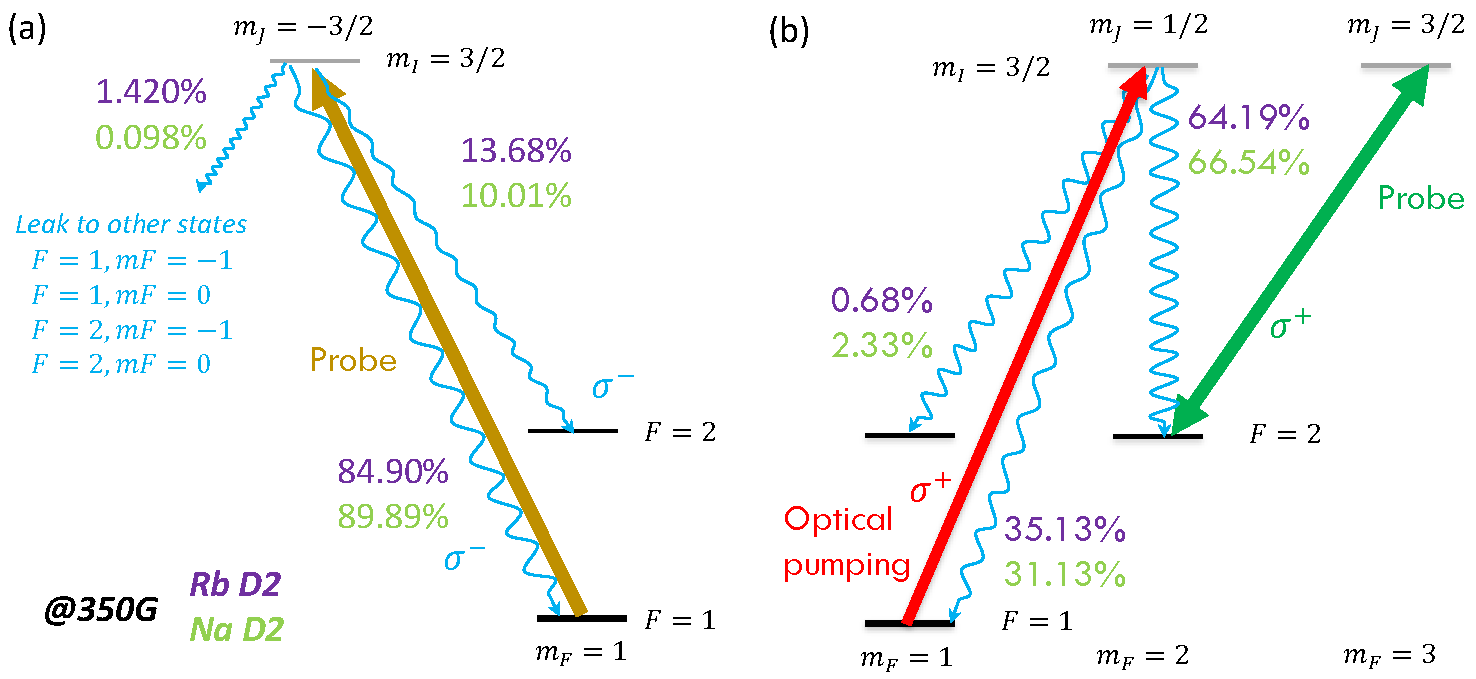
\includegraphics [width = 0.9 \linewidth]{image_scheme_II.pdf}
\end{center}
\caption[Two image schemes for Na(Rb) $\ket{F=1,m_F=1}$ state under 350 G]{(a) non-cycling image scheme for Na(Rb) $\ket{F=1,m_F=1}$ state. (b) After partially pumping the $\ket{F=1,m_F=1}$ atoms to the cycling transition for $\ket{F=2,m_F=2}$ state. The calculation is under 350 G magnetic field.}
\label{image_scheme_II}
\end{figure}

% non-cycling image method in high field (done 2021年8月17日12:03:41)
In July 2018, We first chose the non-cycling transition with \(90\%\) probability back to the original state. With this imaging method on Na, we get the first signal of a droplet. Even though we know it is not a droplet (since the magnetic field is 350.089G, which is higher than the mean-field collapse boundary 349.978 G). We are very close to the collapse bound. However, due to the limited ToF duration and image resolution, we thought that was the droplet. As shown in Fig. \ref{droplet_signal_Na_first}, this deep attractive double BEC already shows its tiny expansion property. Then, we are encouraged and build the Rb high-magnetic-field (HF) image with the beat locking method. We found it hard to use scheme (a) since the high OD cause the sensitivity of the OD we obtain upon the image duration. So we switch to image scheme (b). 

% non-cycling image for droplet signal (done 2021年8月17日12:04:16)
\begin{figure}[htb]
\begin{center}
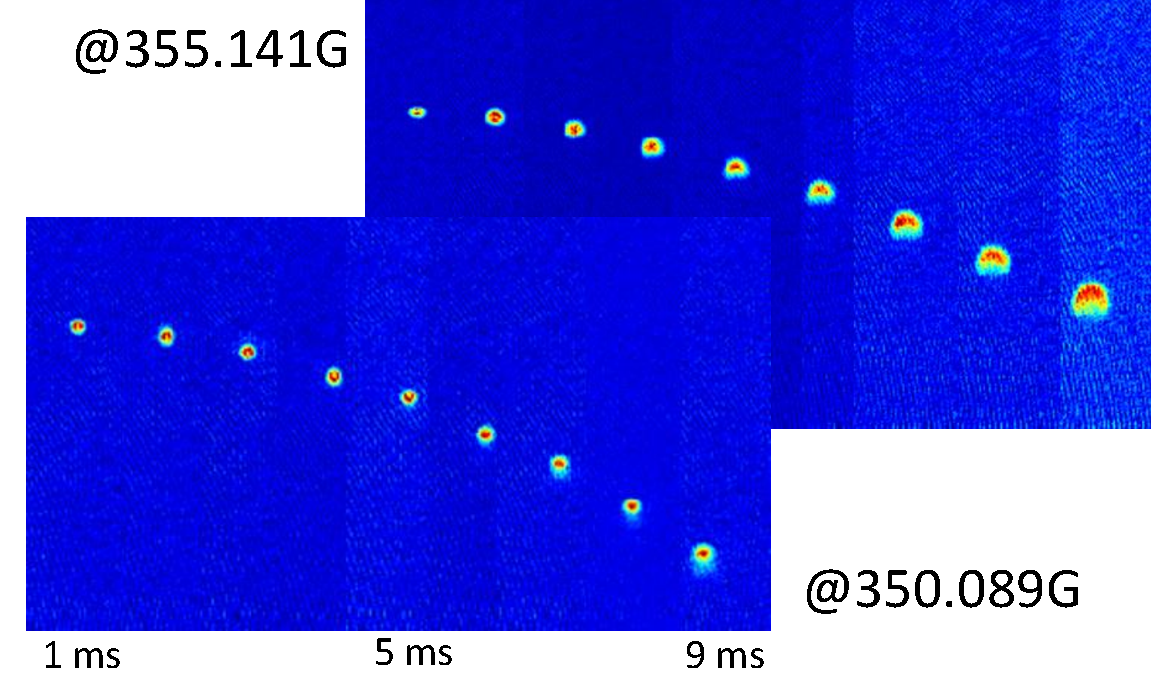
\includegraphics [width = 0.7 \linewidth]{droplet_signal_Na_first.pdf}
\end{center}
\caption[non-cycling absorption image for droplet signal]{Na absorption image with non-cycling scheme. Signal at 350 G show clear size shrinking and shape turning to sphere.}
\label{droplet_signal_Na_first}
\end{figure}

% found magnetic field gradient (done 2021年8月17日12:22:02)
Thanks to images for both species, we discover the magnetic gradient affecting the droplet sample. As shown in Fig. \ref{gradient_compensation}, the gradient applies on Na and Rb generate different forces due to different mass and dipole. The mixture sample tends to be torn apart. So, for observing a better droplet signal without the effect of a gradient, we compensate the gradient with another single-coil (right panel of Fig. \ref{gradient_compensation}). By measuring the accelerations of both Rb and Na, we can choose the best compensation point. After solving this problem, we obtain the non-expansion signal of the droplet clearly, as shown in Fig. \ref{first_signal_both}. We use an imbalanced number case; the Na number is much larger than Rb. A clear, bright spot shows up at the centre of the Na BEC, which shows the smoking-gun signal for the droplet.

% first signal for both case (done 2021年8月16日11:42:23)
\begin{figure}[htbp]
\begin{center}
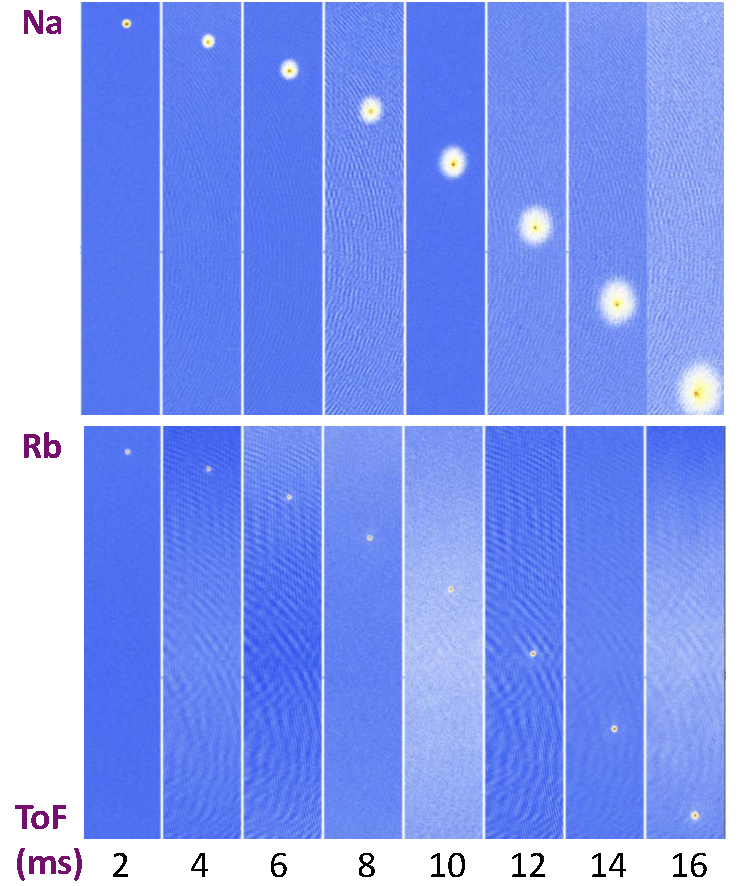
\includegraphics [width = 0.7 \linewidth]{first_signal_both.pdf}
\end{center}
\caption[Droplet signal of number imbalanced case]{Na and Rb droplet signal under 349.826 G. atomic number for Na(Rb) is $9\times10^4$ ($3\times10^4$). A clear, bright spot shows up inside the BEC surrounding of Na sample.}
\label{first_signal_both}
\end{figure}

% signal under 3x image system with Na Rb both partial pump method (done 2021年8月17日12:32:51)
After the detection we made in Fig. \ref{first_signal_both}, we find that the image resolution is limited since the original image system with 3x magnification has a resolution of 4 $\mu$m and pixel corresponding size 2.1 $\mu$m. Both parameters are comparable to the size of the droplet and even larger than it. So, we determined to upgrade our image system. We first choose the set-up of the microscope and the zoom lens system from Navitor. This system offers a magnification changing from 0.8 to 12 times, which is enough for our measurement. Meanwhile, we use a Mitutoyo long-working distance microscope to upgrade the image resolution. After all these upgrades, we achieve a 15x image system with a resolution of around 2 $\mu$m. Details can be found in Sect. \ref{image_system}.

% problem with FR (done 2021年8月17日12:42:35)
In June of 2019, after finishing all the technical problems, we started to take data for the droplet sample. We measured the non-expansion signal and studied the phase diagram. Besides the liquid droplet phase, we also study the gas phase, trying to understand the abnormal expansions. Details can be found in Chap. \ref{Chap_droplet}. Then, we meet the big problem that the experimental measurement of the phase diagram has a 300 mG discrepancy compared to the theoretical calculation. Even we do a more careful compensation of the magnetic field and number calibration, the discrepancy is still there. Finally, we doubt the accuracy of our Feshbach resonance parameter, so we re-do the FR calibration \cite{guo2021tunable}. This is an individual story as depicted in Chap. \ref{Chap_Feshbach}.

% some comments (done 2021年8月17日13:02:27)
I summarize the journey of studying quantum droplets as follows: first, the goal of this study is passive since we did not figure out what we want to study at the very beginning. A clear goal is vital to guide and push the following movement, such as technique upgrading or numerical simulation. Second, the review work done at the first phase is not broad enough. We only focus on the already existing experimental works and theories. Actually, finding the connection between other fields is essential and could guide the following working direction. Third, my attitude to the \textit{numbers} is not serious that caused using of the unverified parameters. This pulled our leg for a long time and finally causing the degrading of this work. In all, it is a good lesson to not only my research career but also to my daily life, from the attitude to details to the way of thinking and doing.

\section{Quantum depletion and Lee-Huang-Yang correction}
\label{sec:intro-LHY}

% Why discuss quantum depletion here (done 2021年8月17日13:20:01)
Back to the motivation of studying quantum droplets, the essential ingredient is the beyond-mend-field effect in a Bose condensate,i.e. the Lee-Huang-Yang (LHY) correction. LHY correction was first introduced by Lee, Huang and Yang in 1957~\cite{lee1957}, as the first-order correction of the ground state of Bose-Einstein condensate. However, due to its mighty contribution, we typically can ignore it. However, when the zero-order mean-field energy is approaching zero, which means the LHY correction could compare to the MF energy or even dominant the sample, we need to treat it more seriously. This section introduces the quantum depletion and LHY correction as a precursor for the next chapter, which discusses the complete theory for the quantum droplet.

% quantum depletion and LHY correction (done 2021年8月17日13:24:47)
Let us consider a Bose-Einstein condensate, with its Hamiltonian as
\begin{equation}
H=\sum_k\epsilon_k\hat{a}_k^\dagger\hat{a}_k+\frac{g}{2V}\sum _{\left\{k_i\right\}}\hat{a}_{k_1}^+\hat{a}_{k_2}^+\hat{a}_{k_3}\hat{a}_{k_4}
\end{equation}
By separating the condensate part and quantum fluctuation part, i.e. considering $a_0$ as $\sqrt{N}$ and write it away from other creation operators (with $k>0$), we have
\begin{equation}
\begin{split}
H=\frac{g N^2}{2V}&+\sum_{k\neq0}\left(\epsilon_k+gn_0\right)\hat{a}_k\dagger\hat{a}_k+\frac{gN}{2V}\sum_{k\neq0}\left(\hat{a}_k^+\hat{a}_{-k}^++\hat{a}_k\hat{a}_{-k}\right)\\
&+\frac{g\sqrt{N}}{2V}\sum_{k_1+k_2+k_3=0}\left(\hat{a}_{k_1}^+\hat{a}_{k_2}^+\hat{a}_{k_3}+\hat{a}_{k_1}^+\hat{a}_{k_2}\hat{a}_{k_3}\right)+\frac{g}{2V}\sum_{k_i\neq0}\hat{a}_{k_1}^+\hat{a}_{k_2}^+\hat{a}_{k_3}\hat{a}_{k_4}
\end{split}
\end{equation}
Ignore the higher order parts and do the Bogoliubov transition, we can get the diagonalized Hamiltonian as
\begin{equation}
\begin{split}
H\simeq \frac{g N^2}{2V}-\frac{1}{2}\sum _{k\neq 0} \left(\epsilon _k+\frac{g N}{V}-E_k\right)+\sum _{k\neq 0} E_k\hat{\alpha }_k\dagger\hat{\alpha
}_k\\
E_k=\sqrt{\epsilon _k\left(\epsilon _k+\frac{2 g N}{V}\right)}=\sqrt{\frac{\hbar ^2k^2}{2m}\left(\frac{\hbar ^2k^2}{2m}+\frac{2 g N}{V}\right)}
\end{split}
\end{equation}
The first part shows the energy shift (MF shift) for the condensate part. Second part shows summation of the energy of all particles with $k>0$, i.e. the quantum depletion. Third part shows the excitation spectrum of the sample and $E_k$ offers the dispersion of the sample. Now, we only consider the ground state properties, i.e. only consider the first two terms of the Hamiltonian. The fraction of depleted particle is
\begin{equation}
\frac{n_{\text{dp}}}{n}=\frac{8}{3\sqrt{\pi }}\sqrt{n a_S^3}
\end{equation}
where, we can directly read that with increasing of $n a_S^3$, more particles get out of the condensate. Meanwhile, these particles will contribute the LHY correction to ground state energy, i.e.
\begin{equation}
\frac{E_{\text{GS}}^R}{V}=\frac{g n^2}{2}\left(1+\frac{128}{15\pi ^{1/2}} \left(n a^3\right)^{1/2}\right)
\end{equation}
where $a=\left|a_S\right|$. Now, we plot ground state energy when $g>0$
Where we can find the LHY correction is small when density is low and only get important when $n a^3\sim 1$. These correction has been experimentally verified in strongly interacting Bose System \cite{Navon2011}. Thus, we find that this correction beyond mean-field theory increases the energy and increases ``hot'' particles. Moreover, considering the excitation spectrum for $g<0$, you can explain that the high energy excitation(short-wave) cure the unstable system of long-wave-instability, which gives the formation of LHY droplet.

% Historical study of LHY correction
% droplet with LHY correction


\section{Thesis Outline}
\label{sec:intro-outline}
% Outlines tells contents of each chapter (done: 2021年8月16日20:35:16)
Chapter \ref{Chap:theory} will discuss two fundamental conceptions: quantum scattering and the microscopic theory of a mixture of Bose condensate, which we will revisit many times in the following chapters. Chapter \ref{Chap_Apparatus} will introduce the main upgrades of apparatus for the droplet experiment. Chapter \ref{Chap_Feshbach} aims at achieving a precision mapping between scattering length and magnetic field, which is realized by a binding energy measurement of Feshbach molecules. After being armed with this accurate information of interaction, we detailed demonstrate the production of a hetero-nuclear droplet in Chapter \ref{Chap_droplet}. In Chapter \ref{chap_LowD}, we turn to discuss droplets in low dimensions and try to offer a possibility of studying this fancy effect in the experiment. Finally, we summarize the thesis with some outlooks for future directions.

\chapterend
